\cohead{\Large\textbf{Tangentengleichungen}}
\fakesubsection{Tangentengleichungen bestimmen}
Damit eine Gerade \(g(x)=mx+b\) eine Tangente an der Stelle \(x_0\) an das Schaubild einer Funktion \(f(x)\) ist, müssen 2 Bedingungen erfüllt sein:
\begin{tcolorbox}
	\textcolor{loestc}{Die Steigung der Funktion an der Stelle \(x_0\) muss der Steigung der Geraden entsprechen:
		\[m=f'(x_0)\]}
\end{tcolorbox}
\begin{tcolorbox}
	\textcolor{loestc}{Die Funktionswerte der Geraden und der Funktion an der Stelle \(x_0\) müssen gleich sein:
		\[g(x_0)=f(x_0)\]}
\end{tcolorbox}
Beispiel: Bestimme die Tangente an die Funktion \(f(x)=\frac{1}{2}x^2-x-1\) an der Stelle \(x_0=2\).\vspace{0.5cm}
\begin{minipage}{\textwidth}
	\begin{minipage}{0.5\textwidth}
		\begin{enumerate}
			\item Gleiche Steigungen an der Stelle \(x_0=2\):\\
			\\
			\textcolor{loes}{\(f'(x)=x-1\) und damit \(m=f'(2)=1\)}\\
			\\
			\\
			\item Gleiche Funktionswerte an der Stelle \(x_0=2\):\\
			\begin{align*}
				\textcolor{loes}{g(2)}&\textcolor{loes}{=f(2)}\\
				\textcolor{loes}{1\cdot 2+b}&\textcolor{loes}{=\frac{1}{2}\cdot 2^2-2-1}\\
				\textcolor{loes}{2+b}&\textcolor{loes}{=-1\ \vert\ -2}\\
				\textcolor{loes}{b}&\textcolor{loes}{=-3}
			\end{align*}
		\end{enumerate}
		\textcolor{loes}{Damit ergibt sich \(g(x)=x-3\)}
	\end{minipage}
	\begin{minipage}{0.5\textwidth}
		\centering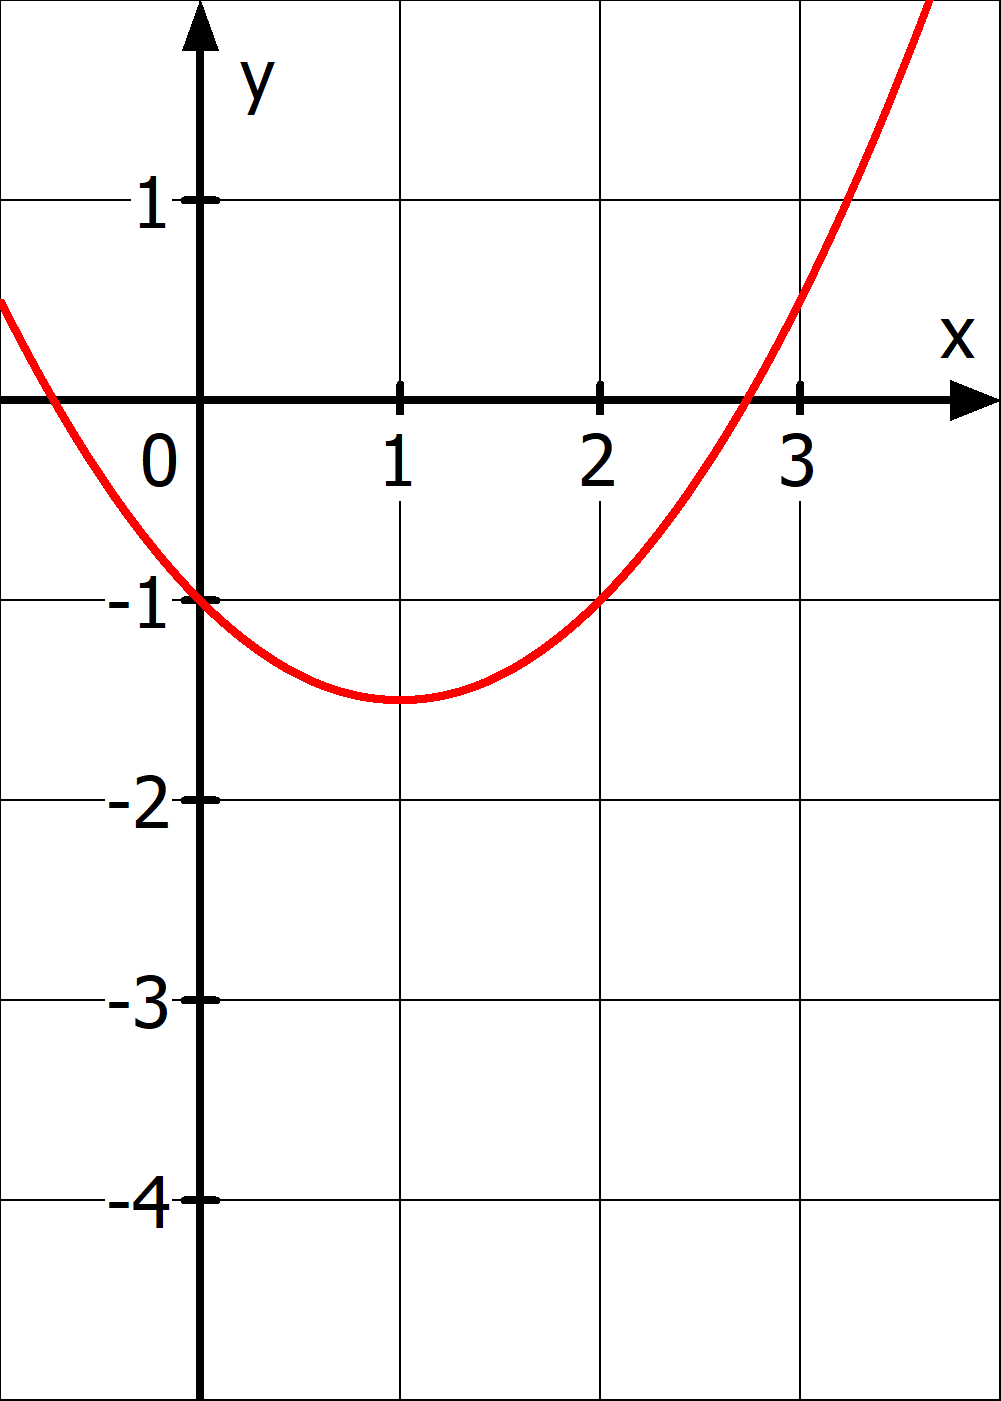
\includegraphics[width=.9\textwidth]{\ableitung/pics/tangenteBsp.png}
	\end{minipage}
\end{minipage}\newpage
%%%%%%%%%%%%%%%%%%%%%%%%%%%%%%%%%%%%%%%%%%%%%%%%%%%%%%%%%%%%%%%%%%%%%%%%%%%%%%%%%%%%%%%%%%%%%%%%%%%%%%%
\begin{Exercise}[title={\raggedright Bestimme jeweils die Tangentengleichung.}, label=tangentenBestimmenA1]
	\begin{enumerate}[label=\alph*)]
		\item \(f(x)=x^2+3\) an der Stelle \(x_0=1\)
		\item \(f(x)=-2x^2+x\) an der Stelle \(x_0=-2\)
		\item \(f(x)=x^3-4\) an der Stelle \(x_0=-1\)
		\item \(f(x)=2x^2-2x\) an der Stelle \(x_0=0\)
		\item \(f(x)=0,25x^4-x^2\) an der Stelle \(x_0=3\)
		\item \(f(x)=x^2-2x+4\) an der Stelle \(x_0=-3\)
		\item \(f(x)=x^3-x^2+x\) an der Stelle \(x_0=3\)
		\item \(f(x)=\frac{1}{3}x^3-x+3\) an der Stelle \(x_0=2\)
		\item \(f(x)=e^x\) an der Stelle \(x_0=\ln(2)\)
		\item \(f(x)=-3e^{2x}\) an der Stelle \(x_0=\ln\left(\frac{1}{2}\right)\)
		\item \(f(x)=\frac{3}{8}x^4-\frac{3}{4}x^2-x\) an der Stelle \(x_0=-1\)
		\item \(f(x)=\frac{1}{2}x^2-5x+6\) an der Stelle \(x_0=6\)
		\item \(f(x)=-3e^{2x}\) an der Stelle \(x_0=\ln(3)\)
		\item \(f(x)=\frac{3}{2}e^{0,5x}-3\) an der Stelle \(x_0=\ln(9)\)
		\item \(f(x)=-\frac{3}{16}x^4+\frac{5}{12}x^3+\frac{3}{4}x\) an der Stelle \(x_0=-2\)
	\end{enumerate}
\end{Exercise}
%%%%%%%%%%%%%%%%%%%%%%%%%%%%%%%%%%%%%%%%%
\begin{Answer}[ref=tangentenBestimmenA1]\\
	\begin{enumerate}[label=\alph*)]
		\item \(g(x)=2x+2\)
		\item \(g(x)=9x+8\)
		\item \(g(x)=3x-2\)
		\item \(g(x)=-2x\)
		\item \(g(x)=21x-\frac{207}{4}\)
		\item \(g(x)=-8x+5\)
		\item \(g(x)=22x-45\)
		\item \(g(x)=3x-\frac{7}{3}\)
		\item \(g(x)=2x+2-2\ln(2)\)
		\item \(g(x)=-\frac{3}{2}x-\frac{3}{4}-\frac{3}{2}\ln(2)\)
		\item \(g(x)=-\frac{61}{6}x-\frac{29}{4}\)
		\item \(g(x)=x-12\)
		\item \(g(x)=-54x-27+54\ln(3)\)
		\item \(g(x)=\frac{9}{4}x+\frac{3}{2}-\frac{9}{4}\ln(9)\)
		\item \(g(x)=\frac{47}{4}x+\frac{47}{3}\)
	\end{enumerate}
\end{Answer}